\documentclass[12pt,a4paper]{report}

%----------------------------------------------------------------------------------------
%   PACKAGES
%----------------------------------------------------------------------------------------
\usepackage[francais]{babel} % French language package
\usepackage[utf8]{inputenc} % UTF8
\usepackage[T1]{fontenc} % acute french accents
\usepackage[pdftex]{graphicx} % figures
\usepackage{hyperref} % hyperlinks
\usepackage[dvipsnames]{xcolor} % colors
\usepackage{amsthm} % mathematical symbols
\usepackage{natbib} % To add the bibligraphy
\usepackage[page,toc,titletoc,title]{appendix} %To add appendices to the document
\usepackage[nottoc,notlot,notlof]{tocbibind} %To bind the table of contents to the bibligoraphy
\usepackage{titlesec}
\titleformat{\chapter}[display]
{\normalfont\huge\bfseries}{\chaptertitlename\ \thechapter}{20pt}{\Huge}
\titlespacing*{\chapter}{0pt}{-50pt}{40pt}

\makeatletter
\setlength{\@fptop}{0pt}
\makeatother

\hypersetup{
    colorlinks,
    linkcolor={red!50!black},
    citecolor={blue!50!black},
    urlcolor={blue!80!black}
}

\newcommand{\HRule}{\rule{\linewidth}{0.5mm}} % Defines a new command for the horizontal lines

\theoremstyle{definition}
\newtheorem*{definition}{Définition}
\newtheorem{example}{Exemple}
\newtheorem*{remark}{Remarque}

\begin{document}
\pagenumbering{roman}
%----------------------------------------------------------------------------------------
%   TITLE PAGE
%----------------------------------------------------------------------------------------
\begin{titlepage}
\center

%----------------------------------------------------------------------------------------
%   LOGOS SECTION
%----------------------------------------------------------------------------------------

\includegraphics[scale=0.5]{images/umLogo.png} % Université de Montpellier Logo
\hspace{\fill}

\includegraphics[scale=0.25]{images/fdsLogo.jpg} % Faculté de Sciences Logo

%----------------------------------------------------------------------------------------
%   HEADING SECTIONS
%----------------------------------------------------------------------------------------
\textsc{\LARGE M1 Informatique AIGLE}\\[1cm]
\textsc{\Large \textbf{HMIN201}}\\[0.25cm]
\textsc{\large M1 TER}\\[0.5cm]

%----------------------------------------------------------------------------------------
%   TITLE SECTION
%----------------------------------------------------------------------------------------
\HRule \\[0.4cm]
{ \huge \bfseries TER: Software Heritage}\\[0.4cm]
{ \Large \bfseries Rapport Final}\\[0.4cm]
\HRule \\[0.5cm]

%----------------------------------------------------------------------------------------
%   AUTHORS AND SUPERVISORS SECTION
%----------------------------------------------------------------------------------------
{ \huge \bfseries Groupe \textsc{Bajonim}}\\[0.4cm]
\begin{minipage}{0.4\textwidth}
\centering \small
\textbf{Bachar \textsc{Rima}}, \\ \href{mailto:bachar.rima@etu.umontpellier.fr}{bachar.rima@etu.umontpellier.fr}\\ % Student
\textbf{Joseph \textsc{Saba}}, \\ \href{mailto:joseph.saba@etu.umontpellier.fr}{joseph.saba@etu.umontpellier.fr}\\ % Student
\textbf{Tasnim \textsc{Shaqura}}, \\ \href{mailto:tasnim.shaqura@etu.umontpellier.fr}{tasnim.shaqura@etu.umontpellier.fr}\\ % Student
\end{minipage} \\[0.8cm]

\begin{minipage}[b]{0.4\textwidth}
\begin{flushleft} \large
\emph{Encadrant:} \\
Jessie \textsc{Carbonnel} % Academic Supervisor
\end{flushleft}
\end{minipage}
~
\begin{minipage}[b]{0.4\textwidth}
\begin{flushright} \large
\emph{Responsable de l'UE:} \\
Mattieu \textsc{Lafourcade} % UE Supervisor
\end{flushright}
\end{minipage}\\[1.5cm]

%----------------------------------------------------------------------------------------
%   DATE SECTION
%----------------------------------------------------------------------------------------
{\large 27 mai 2019}\\[1cm]
\hspace{\fill}
\vfill % Fill the rest of the page with whitespace
\end{titlepage}

%----------------------------------------------------------------------------------------
%   INTRODUCTION
%----------------------------------------------------------------------------------------
\tableofcontents
\cleardoublepage

\pagenumbering{arabic}
\setcounter{page}{1}
\chapter{Introduction}
Les logiciels sont actuellement omniprésents dans tous les aspects de notre vie quotidienne; ils constituent l'un des piliers de l'héritage humain et doivent être préservés contre toute suppression et tout endommagement. Archiver leurs codes source s'avère ainsi une tâche primordiale. En effet, le code source d’un logiciel constitue un artefact logiciel essentiel dans le domaine des connaisances scientifiques, culturelles, et techniques. D’autre part, le code source est facilement lisible et compréhensible par les humains, et peut être transformé en fichiers exécutables. À ce titre là, des plateformes ont déjà été proposées telles que \href{https://archive.org/}{\texttt{The Internet Archive}} et \href{https://unescopersist.org/}{\texttt{UNESCO Persist}}. Toutefois, ces plateformes se concentraient plutôt sur la préservation des fichiers exécutables au lieu du code source \textsuperscript{\citep{internetArchive}}\textsuperscript{\citep{unescoPersist}}.

\section{Description de Software Heritage}
\texttt{Software Heritage} est une initiative lancée par \textbf{INRIA}\textcolor{RoyalBlue}{\footnote{\textbf{Institut National de Recherche en Informatique et Automatique}}}, soutenue par l'\textbf{UNESCO} et visant \og la collecte, la conservation et le partage de code source de tous les logiciels publiquement accessibles depuis n'importe quelle plateforme d'hébergement de code source \fg \textsuperscript{\citep{dicosmoWhyAndHow}}.

Son architecture consiste en un \textit{framework} permettant de retrouver le code source des logiciels susmentionnés et de les ingérer au sein de l’archive universel de \texttt{Software Heritage}. En particulier, les \textbf{Listers} en constituent une partie centrale: il s’agit de \textit{crawlers} configurés pour parcourir des dépôts de code source, \og \textit{mapper} \fg~ leurs modèles à des modèles intégrables à l'infrastructure, et reporter l'ingestion de leur contenu à d’autres composants du \textit{framework}. L'ingestion du contenu d'un dépôt \og \textit{listé} \fg au sein de l'archive est effectuée par des composants spécifiques, les \textbf{Loaders}. Enfin, la planification des tâches du \textit{listing} et du \textit{loading} est régulée par un \textbf{Scheduler}, un composant interagissant avec une queue de tâches asynchrones opérée par un serveur \texttt{Celery}.

Il faut préciser que les plateformes d’hébergement embarquent chacune des dépôts de code source à structures différentes, ce qui nécessite la création d’un \textbf{Lister} dédié pour chaque plateforme. Par ailleurs, les différentes versions d'un logiciel et leurs métadonnées associées sont gérées par un gestionnaire de version, ce qui nécessite la création d'un \textbf{Loader} dédié pour chaque gestionnaire. Actuellement, tous les \textbf{Listers} et \textbf{Loaders} ont été créés uniquement par l’équipe de \texttt{Software Heritage}. Les \textbf{Listers} développés l'ont été pour les plateformes d’hébergement les plus populaires (\texttt{Github}, \texttt{Bitbucket}, $\dots$). De même, les \textbf{Loaders} développés l'ont été pour les gestionnaires de version les plus populaires (\texttt{Git}, \texttt{SVN}, \texttt{Mercurial}, $\dots$).

\section{Contexte du TER}
Dans le cadre de ce projet, encadré par Jessie Carbonnel, du module \textbf{HMIN201} désignant le TER, encadré par Mathieu LaFourcade, notre objectif final consiste à créer un \textbf{Lister} pour une plateforme de développement ciblée. Ainsi, les tâches nécessaires à effectuer afin d'accomplir ce but peuvent être énumérées de la manière suivante :
\begin{itemize}
	\item Lire et comprendre les articles et tutoriels écrits par l’équipe de \texttt{Software Heritage} ;
	\item Analyser différentes plateformes d’hébergement afin d’en cibler une ;
	\item Concevoir et développer un \textbf{Lister} pour la plateforme choisie ;
	\item Répliquer localement l’environnement de \texttt{Software Heritage} afin de tester le \textbf{Lister} développé ;
	\item Faire une \textit{Pull Request} afin d’intégrer le \textbf{Lister} testé au dépôt de développement de \texttt{Software Heritage} sur \texttt{GitHub}.
\end{itemize}

\section{Plan du rapport}
Nous commençons ce rapport par une courte description de \texttt{Software Heritage}, suivie par la spécification du contexte du stage. Ensuite, nous détaillerons la problématique générale traitée par \texttt{Software Heritage} et la sous-problématique particulière adressée par notre projet.

Par la suite, nous fournirons une explication technique détaillée de l'infrastructure de \texttt{Software Heritage} et de son fonctionnement, l'étape fondamentale sur laquelle se base notre méthodologie, et nous terminerons la section par le planning prévisionnel du projet. Après, nous élaborerons nos approches pour la conception d'un \textbf{Lister} et son implémentation, ainsi que les résultats obtenus.

Pour conclure, nous comparerons les versions prévisionnelle et finale du planning, puis nous discuterons les difficultés rencontrées et les perspectives du projet. Finalement, nous listerons un bilan du projet en citant ses apports.


\chapter{Problématique}
Les logiciels sont actuellement omniprésents dans tous les aspects de notre
vie quotidienne; archiver leurs codes source paraît ainsi une tâche primordiale. À ce titre là, des plateformes ont déjà été proposées, telles que The Internet Archive
et UNESCO Persist. Toutefois, ces plateformes se concentraient plutôt sur la
préservation des fichier exécutables; allant jusqu'à offrir des émulateurs pour permettre l'éxecution des logiciels présents dans leurs archives.
Par comparaison, Software Heritage s'interesse au code source des logiciels, pas à leurs éxecutables. En effet, le code source d'un logiciel constitue un artefact logiciel fondamental dans le domaine des connaisances scientifiques, culturelles, et techniques. Le code source est écrit sous une forme compréhensible par les humains, et peut façilement être transformé en une forme éxecutable par une machine. Le code source est muable et évolue celon les besoins. Ca préservation nous permet d'accéder à l'historique du developement d'un logiciel.

Malgrés son importance dans notre vie quotidienne, il est façile de voir que nous prennons pas soin correctment du code source. Cela est dû à trois raisons principales.

\section{La diaspora du code source}
Le quantité de projets open sources a vu un énorme accroissement pendant les deux dèrnieres décennies. Le code source de ces projets sont souvent développés sur des plateformes d'hébergement publiques(comme \textit{Github} et \textit{BitBucket}), ou sur des divers forges institutionelles.
Beaucoup d'options s'offrent aux développeurs pour distribuers leurs logiciels. La distribution peut se faire sur des plateforms comme \textit{Github}. Elle peut se faire via des archives liés à des ecosystemes spécifiques, comme \textit{CTAN}, qui distribue des logiciels pour TeX. Les développeurs peuvent aussi choisir de publier leurs logiciels sur des distributions comme \textit{Debian} et \textit{Fedora}, ou via un gestionaire de paquets comme \textit{npm} et \textit{pip}.
\section{La fragilité du code source}
Le code source est une entité fragile. Elle peut être façilement détruite ou perdue si elle n'est pas fréquement sauvegardée. Les plateforms d'hébergement ne guarantient pas forcement la préservation de leurs contenus; des grandes plateformes d'hébergement ont déja arreter leurs services.
\section{Software Heritage en tant que solution}
	Software Heritage a été créer pour relever ces défis. Software Heritage vise a fournir une infrstructure qui permet la collection, l'organisation, le préservation, et l'accés à tout code source publique. L'archive doit avoir la capacité d'accomplir ses objectifs pour toutes plateformes de dévelopement et de distribution, et doit pouvoir persister les codes source sur le long terme.

	\textbf{Current status et roadmap de SWH}
\section{Les défis}
\textbf{Identifier les plateformes d'hébergement :} Les projets peuvent être hébergés sur des plateformes bien connues, comme sur des plateformes obscures. Il faut construire un catalog des plateformes.
\textbf{Supporter differents protocoles : } Software Heritage doit pouvoir recupérer leurs projets et doit pouvoir maintenir les modifications faites sur ces projets. Vu qu les plateformes d'hébergements sont hétérogènes, Software Heritage essayera de promouvoir des bonnes pratiques pour le préservation.
\textbf{Parcourir les historiques de développement :} Les plateformes d'hébergements supportent differents logiciels de gestion de versions qui n'ont pas les même modèles de données. Software Heritage construira un tel modèle unifiant.
\section{Les principes de base}
\subsection{Transparence et gratuité}
Pour pouvoir assurer la préservation de l'archive sur le long terme, il faut que tout les élements formant l'archive soient open source et accessibles au publique.
\subsection{Réplication compréhensive de l'entiereté du système}
Un tel archive est soumis à differents types de risques. Ces risques étant inévitables, le système doit pouvoir les tolérer. Le système sera répliqué sur differents niveaux: differentes localisations géographiques, differents matériels de stockage , etc...
\subsection{Multitude des partenaires, sans profits}
Pour atteindre ses objectifs, Software Heritage ne doit pas dépendre sur une seule entité qui cherche d'en profiter, et ne doit pas être créer pour la géneration de profits. Ce projet doit apporter de la valeur au public en large, et non seulement pour les organisations qui le supporte.
\subsection{Pas de présélection}
 Il est impossible de savoir quel projets vont finir par être les plus importants. Il faut doc préserver tout les logiciels disponibles sans présélection, surtout que la capacité technique de faire cela est disponible.
\subsection{Source Code First}
Bien qu'il est intéressant de garder le contexte du code source (comme les Wiki, l'environement où le programme est éxécuté, etc), une telle tâche nécessite une énorme quantité de resources, surtout qu'il n'y a pas de préselection. Software Heritage se contente d'archiver les code sources ainsi que leur historique de développement capturé par les logiciels de gestion de versions. Cela permet de guarder des informations importantes qu'on retrouve dans les messages de commit.
\subsection{Identifiants Intrinsèque}
Les identifiants des objets stockés ne doivent pas dépendre des sources externes et doivent pouvoir être calculés à partir des objets qu'ils identifient. Ils sont étroitement liés à ces objets. Cela permet de verifier que l'objet obtenu correspond à l'objet demandé, et permet la détection les modifications sur l'objet.
\subsection{Informations de provenance et informations factuelles}
Software Heritage va stocké les informations de provenance qui décrivent le ou, le quoi, et le quand des objets dans l'archive. Ces informations vont être verifiés et les méthodes de verification vont être stockées aussi.
\subsection{Minimalisme}
Software Heritage se contentera de construire l'infrastructure essentielle et rien de plus.
\section{Notre travail}
Dans le cadre de ce projet, encadré par Jessie Carbonnel, nous avons cibler la plateforme d'hébergement Launchpad afin de collectioner les codes sources qui y sont hébergés, et les stocker dans l'archive de Software Heritage. Ainsi, les objectifs de ce TER peuvent être énumérés de la manière suivante :
\begin{itemize}
\item Lire/comprendre les articles et tutoriels écrits par l'équipe de Software Heritage;
\item Analyser différentes plateformes d'hébergement afin d'en cibler une;
\item Concevoir et développer un Lister pour la plateforme choisie;
\item Répliquer localement l'environnement de Software Heritage afin de tester le Lister développé;
\item Faire une Pull Request afin d'intégrer le Lister testé au dépôt de développement de Software Heritage.
\end{itemize}

\chapter{Analyse}
\section{Terminologie et fonctionnement de Software Heritage}
\subsection{Modèle des données}
Le modèle des données de \texttt{Software Heritage} est centré sur la notion de stockage d'\og \textbf{artefacts logiciels} \fg~ et leurs \textbf{informations de provenance} correspondantes, hébergés sur des \textbf{plateformes d'hébergement de code source}\textsuperscript{\citep{dicosmoWhyAndHow}}.

\subsubsection{Plateformes d'hébergement de code source}
Les \textbf{plateformes d'hébergement de code source} sont destinées à être \og \textit{crawlées} \fg~ par des \textbf{Listers} et ingérées au sein de l'archive universel de \texttt{Software Heritage} par des \textbf{Loaders}\textsuperscript{\citep{dicosmoWhyAndHow}}. Ces plateformes sont catégorisées de la manière suivante :
\begin{description}
	\item [\textit{forges} de développement collaboratif :] \texttt{GitHub}, \texttt{GitLab}, \texttt{BitBucket}, $\dots$
	\item [dépôts d'un gestionnaire de paquets :] \texttt{PyPI}\footnote{\textbf{\textit{Python Package Index}}}, \texttt{CPAN}\footnote{\textbf{\textit{Comprehensive Perl Archive Network}}}, \texttt{npm}\footnote{\textbf{\textit{Node Package Manager}}}, $\dots$
	\item [distributions logicielles FOSS\footnotemark :]\footnotetext{\textbf{\textit{Free and Open-Source Software}}} \texttt{Debian}, \texttt{Fedora}, \texttt{FreeBSD}, $\dots$
	- other types: e.g.
	\item [autres :] par exemple les \textbf{URL}s\footnote{\textbf{\textit{Uniform Resource Locator}}} personnelles et celles désignant des collections de projets institutionnels non hébergées sur des \textit{forges}.
\end{description}

\subsubsection{Artefacts logiciels}
\begin{definition}[\textbf{Artefact Logiciel}]\mbox{}\\
Selon \href{http://www.granddictionnaire.com/ficheOqlf.aspx?Id_Fiche=8367467}{Le grand dictionnaire terminologique}, un \textbf{artefact logiciel} désigne tout \og \textit{module d'information utilisé ou produit lors de la conception d'un logiciel} \fg.
\end{definition}

Dans le cadre de \texttt{Software Heritage}, pour tout logiciel hébergé sur une plateforme d'hébergement de code source, il existe plusieurs \textbf{artefacts logiciels} qui sont assez récurrent lors du développement du logiciel, et qui constituent les composants de base de l'archive\textsuperscript{\citep{dicosmoWhyAndHow}}. Ces artefacts peuvent être catégorisés de la manière suivante :
\begin{enumerate}
	\item \textit{file contents} ou \textit{blobs} ;
	\item \textit{directories} ;
	\item \textit{revisions} ou \textit{commits} ;
	\item \textit{releases} ou \textit{tags}.
\end{enumerate}

\begin{definition}[\textbf{Blob}]\mbox{}\\
Le \textbf{contenu binaire du code source} (\textit{i.e. les octets}), sans aucune métadonnée associée (même pas le nom du blob). C'est Un artefact récurrent à travers différentes versions d'un même logiciel, différents répertoires du même projet, voire même différents projets.
\end{definition}

\begin{definition}[\textbf{Directory}]\mbox{}\\
Une \textbf{liste récursive d'entrées nommées} pointant vers d'autres aretfacts (\textit{i.e. des blobs ou d'autres directories}). C'est Un artefact associé à des métadonnées divers (\textit{e.g. bits de permission, estampilles de modification, $\dots$}).
\end{definition}

\begin{definition}[\textbf{Revision}]\mbox{}\\
Une \textbf{version du \textit{directory} racine du logiciel} tel qu'il est capturé par un \textbf{gestionnaire de version} (\textit{i.e. un commit}), contenant la totalité du \textbf{code source} du projet désigné par le logiciel. C'est un artefact associé à des métadonnées divers (\textit{e.g. message de commit, estampilles, versions précédentes, $\dots$}).
\end{definition}

\begin{definition}[\textbf{Release}]\mbox{}\\
Une \textbf{revision stable} qui pourra être mise en production (\textit{i.e. un project milestone}). C'est un artefact associé à des métadonnées divers désignant les \textbf{métadonnées d'une revision} et d'autres (\textit{e.g. nom du release, version du release, signatures digitales, $\dots$}).
\end{definition}

\subsubsection{Informations de provenance des données}
Dans le cadre de \texttt{Software Heritage}, pour tout logiciel hébergé sur une plateforme d'hébergement de code source, les \textbf{informations retournées} par le \textit{crawling} de celui-ci sont appelées les informations de provenance (\textit{provenance information})\textsuperscript{\citep{dicosmoWhyAndHow}}. Ces informations peuvent être catégorisées de la manière suivante :
\begin{enumerate}
	\item \textit{software origins} ;
	\item \textit{projects} ;
	\item \textit{snapshots} ;
	\item \textit{visits}.
\end{enumerate}

\begin{definition}[\textbf{Software Origin}]\mbox{}\\
Un \textbf{ensemble de références} pointant vers les endroits de récupération des \textbf{artefacts logiciels} d'un logiciel, archivés dans \texttt{Software Heritage}. Il s'agit d'une \textbf{paire} $<$\emph{type}, \emph{url}$>$ :
\begin{description}
	\item [type :] le \textbf{type de l'origine} (un \textbf{gestionnaire de version} tel que \texttt{Git} ou \texttt{SVN}, un \textbf{paquet source} tels que \texttt{DSC}\footnote{\textbf{\textit{Debian Source Control}}}, $\dots$)
	\item [url :] une \textbf{adresse URL canonique} désignant l'\textbf{adresse de l'origine} (une \textbf{adresse clonable} par un \textbf{gestionnaire de version}, ou \textbf{téléchargeable} telle qu'un \textit{tarball} téléchargé via \texttt{wget}).
\end{description}
\end{definition}

\begin{definition}[\textbf{Project}]\mbox{}\\
Une \textbf{entité abstraite} associée à des \textbf{software origins} divers, avec leurs métadonnées correspondantes. De plus, un projet peut être \textbf{versionné} et \textbf{imbriqué} dans une \textbf{hiérarchie de projets}, et permet de générer des \textbf{ressources de développement} (\textit{e.g. websites, issue trackers, mailing lists, software origins, $\dots$}).
\end{definition}

\begin{definition}[\textbf{Snapshot}]\mbox{}\\
Une \textbf{snapshot à un instant donné} d'un/plusieurs \textbf{point(s) d'entrée} d'un logiciel référencé par un \textbf{software origin} :
\begin{itemize}
	\item s'il s'agit d'un \textbf{gestionnaire de version} : \textbf{points d'entrée} = les \textbf{branches} de développement (\textit{e.g. une snapshot de la branche principale, une autre snapshot de la branche de features $\dots$}) ;
	\item s'il s'agit d'une \textbf{distribution de paquets source} : \textbf{points d'entrée} = les \textbf{suites}\footnote{différents niveaux de maturité d'un paquet source logiciel} de développement (\textit{e.g. une snapshot pour la dernière version d'un paquet source pour la suite stable}).
\end{itemize}
\end{definition}

\begin{definition}[\textbf{Visit}]\mbox{}\\
Un \textbf{lien} entre un \textbf{software origin} et une \textbf{snapshot}, créé lors de la consultation du \textbf{software origin}, permettant d'enregistrer le \textbf{moment de son consultation} et un \textbf{snapshot entier} de son état.
\end{definition}

\subsubsection{Structure de données}
La structure de données à utiliser pour implanter l'archive doit permettre la déduplication de certains \textbf{artefacts logiciels} et \textbf{informations de provenance} tels que les \textbf{blobs}, les \textbf{directories}, les \textbf{revisions}, les \textbf{releases} et les \textbf{snapshots}. Cette déduplication est essentielle afin d'assurer une préservation à long terme et un stockage efficace. Pour ce faire, \texttt{Software Heritage} ont adopté le modèle d'un \textbf{graphe orienté acyclique Merkel}\textsuperscript{\citep{dicosmoWhyAndHow}} ou \textbf{Merkel DAG}\footnote{\textbf{\textit{Direct Acyclic Graph}}} (cf. Figure \ref{fig:swh_data_structure}).

\begin{figure}[!ht]
	\centering
	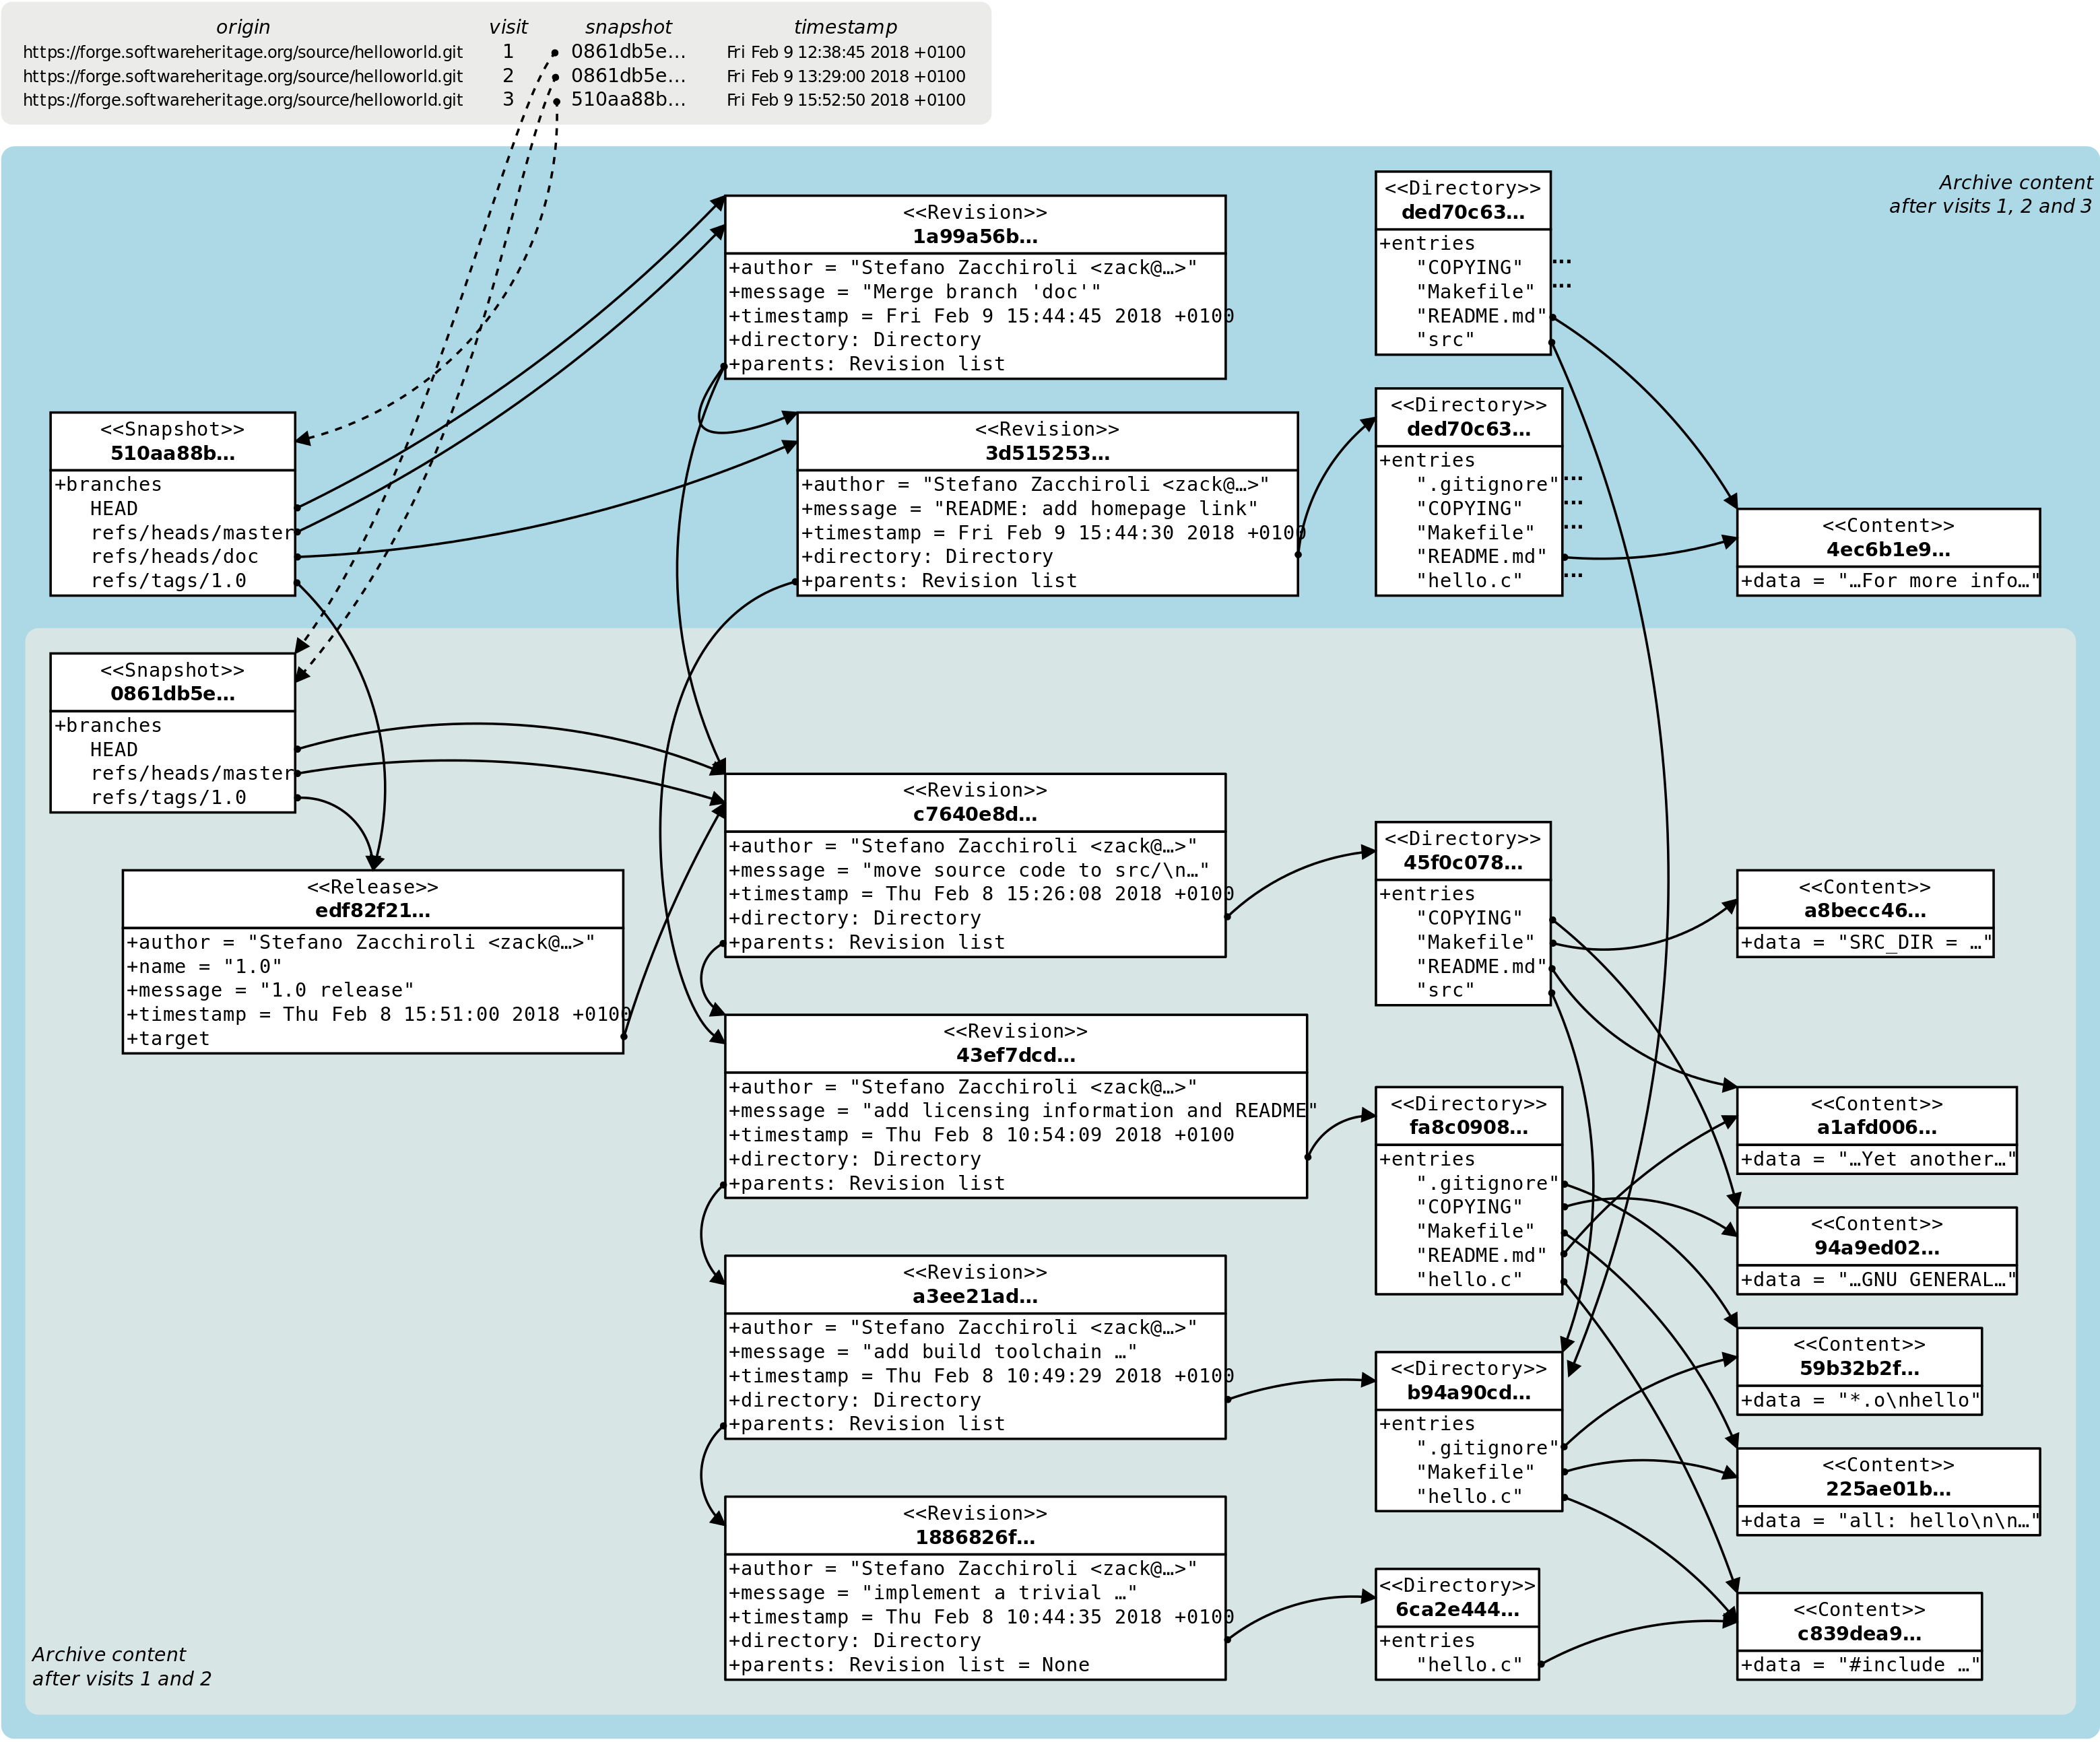
\includegraphics[scale=0.15]{images/swh/data_structure.png}
	\caption{\textbf{Merkel DAG} de \texttt{Software Heritage}\textsuperscript{\citep{swhRevisionNode}}}
	\label{fig:swh_data_structure}
\end{figure}

Le \textbf{Merkel DAG} est composé de noeuds et d'arcs tels que :
\begin{enumerate}
	\item \textbf{noeuds} -- chaque noeud :
	\begin{itemize}
		\item désigne un \textbf{artefact logiciel unique} ;
		\item est identifié par un \textbf{identifieur intrinsèque} désignant un digest cryptographique calculé à partir du noeud et son contenu. Ceci implique qu'un \textbf{software origin} sera ajouté au \textbf{Merkel DAG}, uniquement quand celui-ci ne contient pas déjà un noeud ayant le même identifiant. Cette propriété du \textbf{Merkel DAG} assure une \textbf{déduplication native} à l'archive implanté ;
		\item contient l'ensemble des \textbf{métadonnées} qui lui sont propres (\textit{e.g. messages de commit, estampilles, noms de fichiers, $\dots$}) ;
		\item contient des pointeurs vers les identifiants des \textbf{noeuds enfants} en format canonique.
	\end{itemize}
	\item \textbf{arcs} :
	\begin{itemize}
		\item les \textbf{directories} pointent sur des \textbf{blobs} et d'autres \textbf{directories} ;
		\item les \textbf{revisions} pointent sur des \textbf{directories} et les \textbf{revisions} précédentes ;
		\item les \textbf{releases} pointent sur des \textbf{revisions} ;
		\item les \textbf{snapshots} pointent sur des \textbf{releases} et des \textbf{revisions}.
	\end{itemize}
\end{enumerate}

Un noeud du \textbf{Merkel DAG} désignant une \textbf{revision} est présenté dans la figure \ref{fig:swh_revision_node}. On voit bien l'identifiant intrinsèque du noeud, ainsi que celui du noeud désignant le \textbf{directory racine} pointé par la \textbf{revision}, et celui du noeud désignant la \textbf{revision} précédente. De plus, on voit la date d'ajout, l'auteur, le commiteur, le message et la date du commit de la \textbf{revision}.

\begin{figure}[!ht]
	\centering
	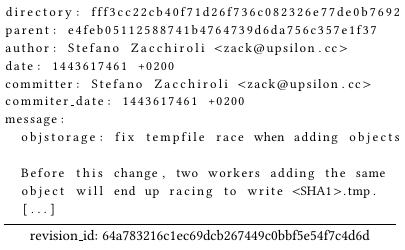
\includegraphics[scale=0.5]{images/swh/revision_node_example.png}
	\caption{Un noeud du \textbf{Merkel DAG} de \texttt{Software Heritage}\textsuperscript{\citep{dicosmoWhyAndHow}}}
	\label{fig:swh_revision_node}
\end{figure}

\subsubsection{Identifieurs intrinsèques}
Afin de pouvoir manipuler les différents \textbf{artefacts logiciels} à archiver, l'archive a besoin de les identifier et de les référencer. Pour ce faire, les identifieurs doivent être uniques, persistents, et intrinsèques. De plus, ils doivent supporter la gestion des versions, ainsi que l'identification à differents niveaux de granularité (\textit{i.e. d'une snapshot à un blob}). Ainsi, l'équipe de \texttt{Software Heritage} a adopté les identifieurs \textbf{IDO}\footnote{\textbf{\textit{Identifiers for Digital Objects}}}, permettant de satisfaire ces besoins\textsuperscript{\citep{dicosmoIDO}}.

Les \textbf{IDO}s sont régis par la \textbf{syntaxe BNF} suivante :
\begin{verbatim}
	<identifier> ::= "swh" ":" <scheme_version> ":" <object_type> ":" <object_id> ;
	<scheme_version> ::= "1" ;
	<object_type> ::=
	"snp" (* snapshot *)
	| "rel" (* release *)
	| "rev" (* revision *)
	| "dir" (* directory *)
	| "cnt" (* content *)
	;
	(* intrinsic object id, as hex-encoded SHA1 *)
	<object_id> ::= 40 * <hex_digit> ;
	<hex_digit> ::= "0" | "1" | "2" | "3" | "4" | "5" | "6" | "7" | "8" | "9"
	| "a" | "b" | "c" | "d" | "e" | "f" ;
\end{verbatim}

Par ailleurs, les \textbf{IDO}s peuvent être complementés par des \textbf{informations contextuelles}, dont deux types sont supportés pour le moment :
\begin{description}
	\item [\textit{origin} :] l'\textbf{URL} \textbf{software origin} du logiciel associé.
	\item [\textit{line numbers of interest} :] le numéro d'une ligne, ou un intervalle.
\end{description}

Les \textbf{informations contextuelles} sont régies par la \textbf{syntaxe BNF} suivante :
\begin{verbatim}
	<identifier_with_context> ::= <identifier> [<lines_ctxt>] [<origin_ctxt>] ;
	<lines_ctxt> ::= ";" "lines" "=" <line_number> ["-" <line_number>] ;
	<origin_ctxt> ::= ";" "origin" "=" <url> ;
	<line_number> ::= <dec_digit> + ;
	<url> ::= (* RFC 3986 compliant URLs *) ;
\end{verbatim}

Les tables \ref{tab:IDO_examples} et \ref{tab:IDO_contextual_examples}, contiennent un ensemble d'exemples d'\textbf{IDO}s avec/sans des informations contextuelles pour différents types de noeuds du \textbf{Merkel DAG}.

\begin{table}[!ht]
	\centering
	\begin{tabular}{|c||c|}
		\hline
		\textbf{IDO} & \textbf{Type de Noeud}\\
		\hline
		\texttt{swh:1:cnt:94a9ed024d3859793618152ea559a168bbcbb5e2} & \textbf{blob}\\
		\hline
		\texttt{swh:1:dir:d198bc9d7a6bcf6db04f476d29314f157507d505} & \textbf{directory}\\
		\hline
		\texttt{swh:1:rev:309cf2674ee7a0749978cf8265ab91a60aea0f7d} & \textbf{revision}\\
		\hline
		\texttt{swh:1:rel:22ece559cc7cc2364edc5e5593d63ae8bd229f9f} & \textbf{release}\\
		\hline
		\texttt{swh:1:snp:c7c108084bc0bf3d81436bf980b46e98bd338453} & \textbf{snapshot}\\
		\hline
	\end{tabular}
	\caption{Exemples d'\textbf{IDO}s de différents noeuds du \textbf{Merkel DAG} de \texttt{Software Heritage}}
	\label{tab:IDO_examples}
\end{table}

\begin{table}[!ht]
	\centering
	\begin{tabular}{|p{9cm}||p{6cm}|}
		\hline
		\textbf{IDO} & \textbf{Type de Noeud}\\
		\hline
		\texttt{swh:1:cnt:41ddb23118f92d721 8099a5e7a990cf58f1d07fa; origin=https://github.com/chrislgarry$\dots$; lines=64-72/} & \textbf{blob} avec l'\textbf{URL} du \textbf{software origin} et l'\textbf{intervalle des lignes} d'intérêt du code source désigné\\
		\hline
		\texttt{swh:1:dir:c6f07c2173a458d09 8de45d4c459a8f1916d900f; origin=https://github.com/id-Software/Qua$\dots$} & \textbf{directory} avec l'\textbf{URL} du \textbf{software origin}\\
		\hline
	\end{tabular}
	\caption{Exemples d'\textbf{IDO}s avec d'\textbf{informations contextuelles} de différents noeuds du \textbf{Merkel DAG} de \texttt{Software Heritage}}
	\label{tab:IDO_contextual_examples}
\end{table}

\subsection{Architecture conceptuelle et flot des données}
\subsubsection{Flot d'ingestion des données}
\begin{figure}[!ht]
	\centering
	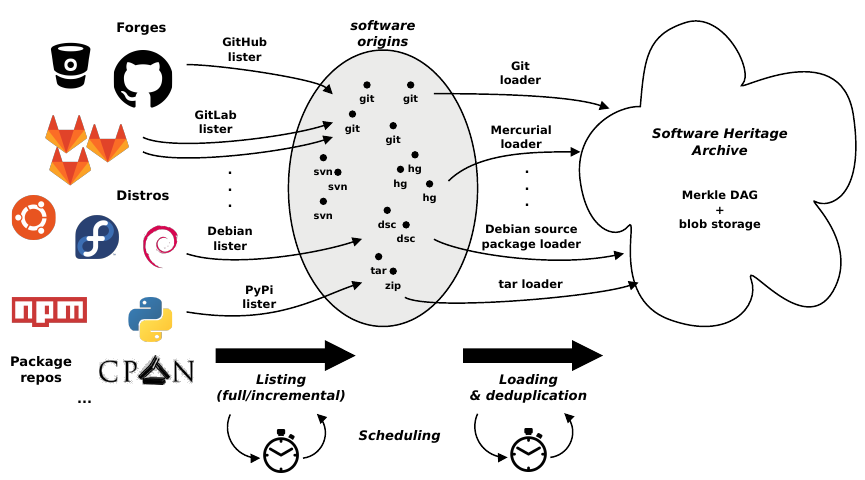
\includegraphics[scale=0.5]{images/swh/conceptual_architecture.png}
	\caption{L'architecture conceptuelle de la plateforme de \texttt{Software Heritage}\textsuperscript{\citep{dicosmoWhyAndHow}}}
	\label{fig:swh_conceptual_architecture}
\end{figure}

L'architecture à adopter pour la plateforme doit permettre de \og \textit{crawler} \fg~ une liste de plateformes d'hébergement de code source et d'archiver leur contenu. Pour ce faire, l'équipe de \texttt{Software Heritage} ont adopté une architecture conceptuelle\textsuperscript{\citep{dicosmoWhyAndHow}} divisant la tâche en deux sous-tâches, effectuées respectivement par deux composants de base: le \textit{listing} des plateformes d'hébergement par des \textbf{Listers} et le \textit{loading} de leur contenu au sein de l'archive de par des \textbf{Loaders} (cf. Figure \ref{fig:swh_conceptual_architecture}).

\subsubsection{Listing}
Le \textit{listing} d'une plateforme d'hébergement de code source consiste à énumérer les \textbf{software origins} qui lui sont associés (e.g. des dépôts sur \texttt{GitHub} ou \texttt{BitBucket}, des paquets source individuels de \texttt{PyPI} ou \texttt{Debian}, $\dots$). Pour chaque plateforme, un \textbf{Lister} dédié doit être créé afin de \og \textit{mapper} \fg les modèles des \textbf{software origins} vers des modèles équivalents intégrables au sein de l'architecture de \texttt{Software Heritage}\textsuperscript{\citep{dicosmoWhyAndHow}}.

En outre, il existe deux techniques de \textit{listing} :
\begin{description}
	\item [\textit{full listing} :] collecter la liste entière des \textbf{software origins} associée à une plateforme d'hébergement de code, afin s'assurer de n'en rater aucun. Il s'agit d'une technique à utiliser une seule fois initialement, et d'une manière moins fréquente ultérieurement en raison de son aspect chronophage, surtout quand la plateforme est relativement grande.
	\item [\textit{incremental listing} :] collecter uniquement l'ensemble des \textbf{software origins} qui ont été modifiés ou ajoutés depuis le dernier \textit{listing}. Il s'agit d'une technique à privilégier et à utiliser régulièrement, suite au premier \textit{full listing}, pour la mise à jour des noeuds correspondant aux \textbf{software origins} au sein du \textbf{Merkel DAG}.
\end{description}

De plus, il existe deux styles de \textit{listing} :
\begin{description}
	\item [\textit{pull style} :] l'archive consulte régulièrement les plateformes d'hébergement de code en vue de lister leurs \textbf{software origins}. Cette technique est assurée par défaut par les \textbf{Listers} apropriés.
	\item [\textit{push style} :] les plateformes d'hébergement collaborant avec \texttt{Software Heritage}, si proprement configurées, notifient l'archive à chaque modification de leurs \textbf{software origins} associés. Cette technique permet de minimiser le décalage entre la version archivée et la version hébergée d'un \textbf{software origin}.
\end{description}

\subsubsection{Loading}
Le \textit{loading} du contenu des \textbf{software origins} d'une plateforme d'hébergement de code, correspond à l'extraction de leurs \textbf{artefacts logiciels} associés et leur ingestion au sein de l'archive. Pour chaque type de \textbf{software origin}, un \textbf{Laoder} dédié doit être créé afin d'\og \textit{ingérer} \fg les \textbf{artefacts logiciels} et \textbf{snapshots} associés, en assurant la contrainte de déduplication des noeuds au sein du \textbf{Merkel DAG}\textsuperscript{\citep{dicosmoWhyAndHow}} (e.g. un \textbf{Loader} pour chaque gestionnaire de version tels que \texttt{Git} ou \texttt{SVN}, un \textbf{Loader} pour chaque format d'un paquet source tels que \texttt{Debian source packages} ou \texttt{tarballs}, $\dots$).

\subsubsection{Scheduling}
Les tâches de \textit{listing} et de \textit{loading} occurrant régulièrement, un composant permettant de planifier leurs occurrences s'avère ainsi primordial. Il s'agit du composant \textbf{Scheduler}, permettant de \textbf{synchroniser} ces tâches dans une \textbf{queue de tâches asynchrones} opérée par un \textbf{serveur} \texttt{Celery}\textsuperscript{\citep{dicosmoWhyAndHow}}.

Le \textbf{Scheduler} est implémenté selon les stratégies d'\textit{adaptive scheduling} et d'\textit{exponential backoff}, s'appuyant la notion d'\textbf{actions fructueuses} ou \textit{fruitful actions}. Ces stratégies permettent d'équilibrer entre la mise à jour du contenu de l'archive et la surcharge des plateformes concernées (\texttt{Software Heritage} et les plateformes d'hébergement de code consultées), surtout lors du \textit{loading} des \textbf{software origins} listés associés à une plateforme assez large.

\begin{definition}[\textbf{Fruitful Action}]\mbox{}\\
Une \textbf{action}, désignant une \textbf{tâche périodique à planifier} (\textit{i.e. listing} ou \textit{loading}), est considérée \textbf{fructueuse}	si la visite associée à l'action retourne de \textbf{nouvelles informations} depuis la \textbf{dernière visite} :
\begin{description}
	\item [\textit{fruitful listing} :] lors de la découverte de nouveaux \textbf{software origins} à \og \textit{lister} \fg~ ;
	\item [\textit{fruitful loading} :] lors du changement de l'état d'un \textbf{software origin} consulté depuis la dernière visite.
\end{description}
\end{definition}

\begin{definition}[\textbf{Adaptive Scheduling and Exponential Backoff}]\mbox{}\\
La \textbf{stratégie} d'\textbf{Adaptive Scheduling} permet d'\textbf{augmenter la fréquence} des visites d'une \textbf{action} quand celle-ci est \textbf{fructueuse}, et de la \textbf{diminuer} dans le cas contraire. Le \textbf{taux} de cette augmentation/diminution est spécifié par la \textbf{stratégie} d'\textbf{Exponential Backoff}, indiquant de le \textbf{doubler} en cas d'une \textbf{augmentation} et de le \textbf{diviser par deux} en cas d'une \textbf{diminution}.
\end{definition}

\subsection{L'archive}
D'une part, la \textbf{conception logique} de l'\textbf{archive} de \texttt{Software Heritage} consiste en un \textbf{Merkel DAG}. D'autre part, l'\textbf{implémentation physique} de l'\textbf{archive} combine plusieurs technologies de stockage, en raison des différentes tailles de stockage des noeuds du \textbf{Merkel DAG}.

\subsubsection{Stockage des noeuds BLOB}
Les \textbf{blobs} occupent la \textbf{majorité de l'espace de stockage}, étant donné qu'ils contiennent la totalité du code source. Afin d'assurer l'espace et les méchanismes de stockage convenables, l'équipe de \texttt{Software Heritage} a introduit un composant \textbf{ObjectStorage} gérant ces tâches\textsuperscript{\citep{dicosmoWhyAndHow}}. Il s'agit d'une \textbf{table de hachage}, associant chaque \textbf{blob} à son \textbf{IDO} correspondant utilisé comme \textbf{clé}. Ceci permet la \textbf{distribution du stockage} dans un \textbf{cluster de tables de hachage} et de profiter des avantages associées.

En cas de \textbf{collision} (\textit{i.e. lorsque le calcul des \textbf{IDO}s de deux objets différents donne un résultat identique}), l'archive utilise plusieurs \textbf{algorithmes de checksum} avec des contraintes d'unicité. Par conséquent, l'archive peut détecter les collisions avant l'ingestion d'un nouvel \textbf{artefact logiciel}. Parmi les algorithmes de checksum utilisé, nous notons \texttt{SHA1} et \texttt{SHA256}.

\subsubsection{Stockage des autres noeuds}
Les autres noeuds du \textbf{Merkel DAG}, notamment les \textbf{directories}, \textbf{revisions}, \textbf{releases} et \textbf{snapshots}, sont stockés chacun dans une \textbf{base de données relationnelle} \texttt{PostgresSQL} dédiée. Chaque \textbf{tuple} d'une table de base de données est identifié par l'\textbf{IDO} du \textbf{noeud correspondant} et contient son contenu\textsuperscript{\citep{dicosmoWhyAndHow}}. Ceci permet la \textbf{distribution du stockage} dans un \textbf{cluster de tables de base de données} et de profiter des avantages associées.

\subsubsection{Réplication des noeuds}
À chaque type de noeud du \textbf{Merkel DAG} est associé un \textbf{log de changement} ou \textit{feed change} persistant, détaillant l'ensemble des \textbf{changements effectués} sur les noeuds\textsuperscript{\citep{dicosmoWhyAndHow}}. Un tel outil est idéal pour la \textbf{réplication} des noeuds: après une opération de \textbf{réplication entière} d'un \textbf{log de changement}, les mirroirs peuvent rester à jour facilement par rapport à l'archive principal par \textbf{réplication incrémentale}.

\subsubsection{Politique de rétention}
La \textbf{politique de retention} permet de \textbf{contrôler la réplication des noeuds}, afin d'assurer un \textbf{système tolérant aux pannes} et la \textbf{longue préservation} des \textbf{artefacts logiciels}\textsuperscript{\citep{dicosmoWhyAndHow}}. Pour ce faire, la politique actuelle précise la nécessité d'avoir deux mirroirs locaux du composant \textbf{ObjectStorage} entier, et une troisième sur un cloud publique. Afin d'assurer le respect de cette politique, un \textbf{composant} de l'infrastructure de \texttt{Software Heritage} :
\begin{itemize}
	\item suit le nombre et la localisation des mirroirs de chaque \textbf{noeud archivé} ;
	\item vérifie régulièrement l'\textbf{adhérence des noeuds archivés} à la \textbf{politique de retention} ;
	\item crée des \textbf{réplications supplémentaires} d'un noeud archivé en cas de manque de mirroirs pour assurer son adhérence à la \textbf{politique de retention}.
\end{itemize}

\subsubsection{Récupération automatique des objects corrompus}
En cas d'un noeud corrompu, un composant de l'infrastructure \texttt{Software Heritage}\textsuperscript{\citep{dicosmoWhyAndHow}} :
\begin{itemize}
	\item choisit \textbf{régulièrement} un ensemble \textbf{aléatoire} de \textbf{noeuds archivés} à \textbf{vérifier} ;
	\item re-calcule l'\textbf{IDO} de chaque noeud de l'ensemble choisi, ainsi que celui de chacun de ses \textbf{mirroirs}, afin de vérifier leur \textbf{intégrité} ;
	\item en cas de \textbf{violation d'une contrainte d'intégrité} par l'une des copies du noeud archivé, tous les mirroirs du noeud concerné seront \textbf{vérifiés dynamiquement}. Au cours de la vérification, les \textbf{versions corrompues} du noeud concerné seront \textbf{automatiquement remplacées} par un \textbf{mirroir} vérifiant la \textbf{contrainte d'intégrité} parmis ceux choisis.
\end{itemize}

\subsection{Architecture technique}

\subsection{Diagrammes de séquence}

\section{Méthodologie}
% Sourceforge sitemap, api\\
% Launchpad api, client\\
% Analyzing the listers (bitbucket, gitlab, github, eclipse, LIRMM, OpenHub, 			Assembla, GNU savannah\\
% heritage, injection de dependances\\
% conclusion: on adoptera une strategie pour definir un lister, loader ou autre\\

\section{Planning Prévisionnel}
\begin{figure}[!ht]
\hspace*{-3.5cm}
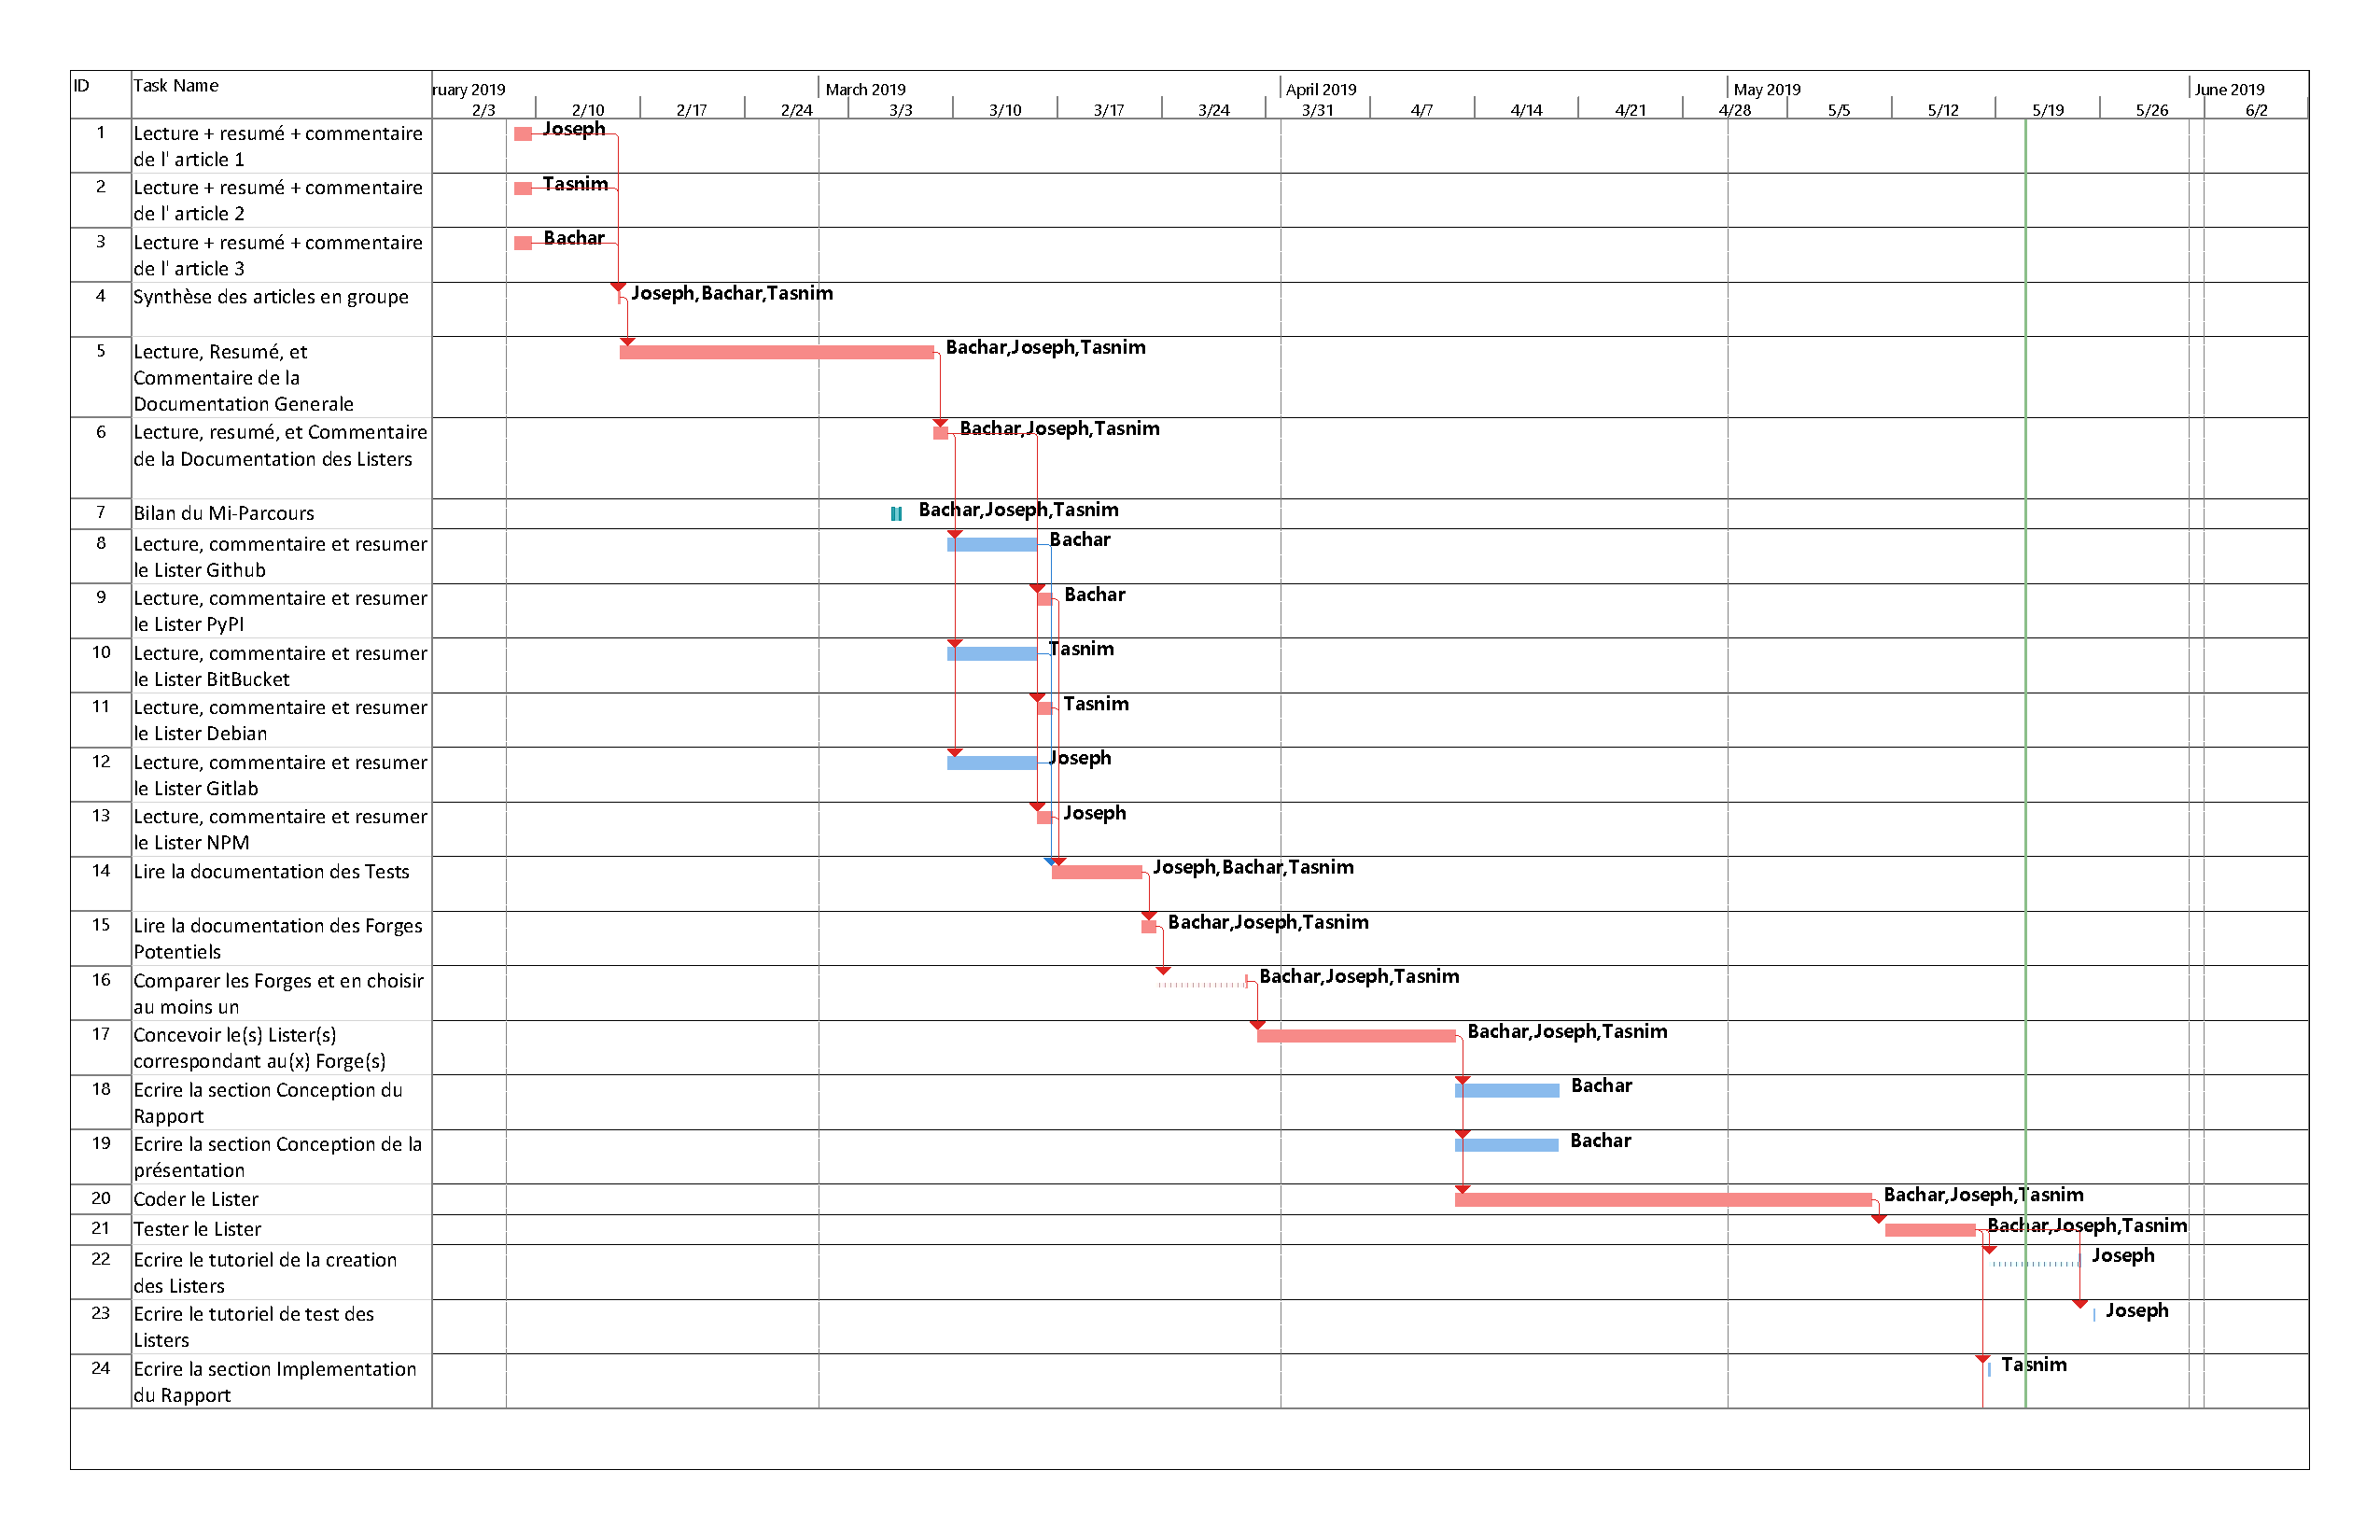
\includegraphics[scale=0.48]{pdfs/feuille_de_route.pdf}
\end{figure}

\begin{figure}[!ht]
\hspace*{-3cm}
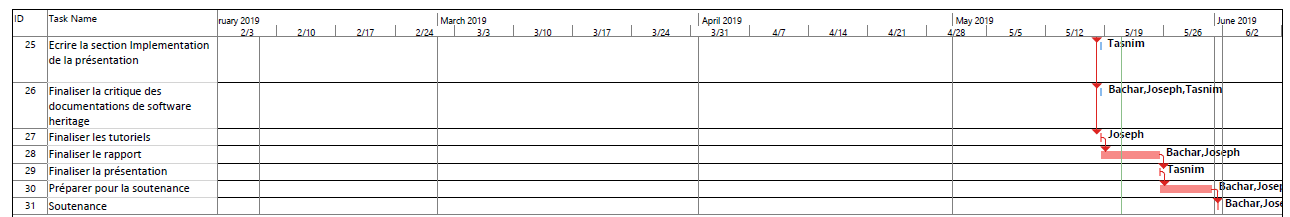
\includegraphics[scale=0.57]{images/planning_prev_p2.PNG}
\caption{Planning prévisionel}
\end{figure}

\chapter{Conception}
design de la solution proposée (diagrammes + explications)

\chapter{Implémentation}
	Les Listers de Software Heritage et les codes qui les accompagnent sont écrits en Python.

	\section{Le client Launchpad}
	les technos qu'on a utilisé\\
	bibliotheques\\
	Outils (e.g. XML parsers)\\
	parler du client
	parler du notebook
	parler du code qu'on a créer par rapport au client (les classes du proxy)
	parler du JSON et de son format, et comment il est mapped to SWH's model

\chapter{Résultats}
pull request?

\chapter{Conclusion}
	\section{Planning final}
	\begin{figure}[!ht]
	\hspace*{-3cm}
	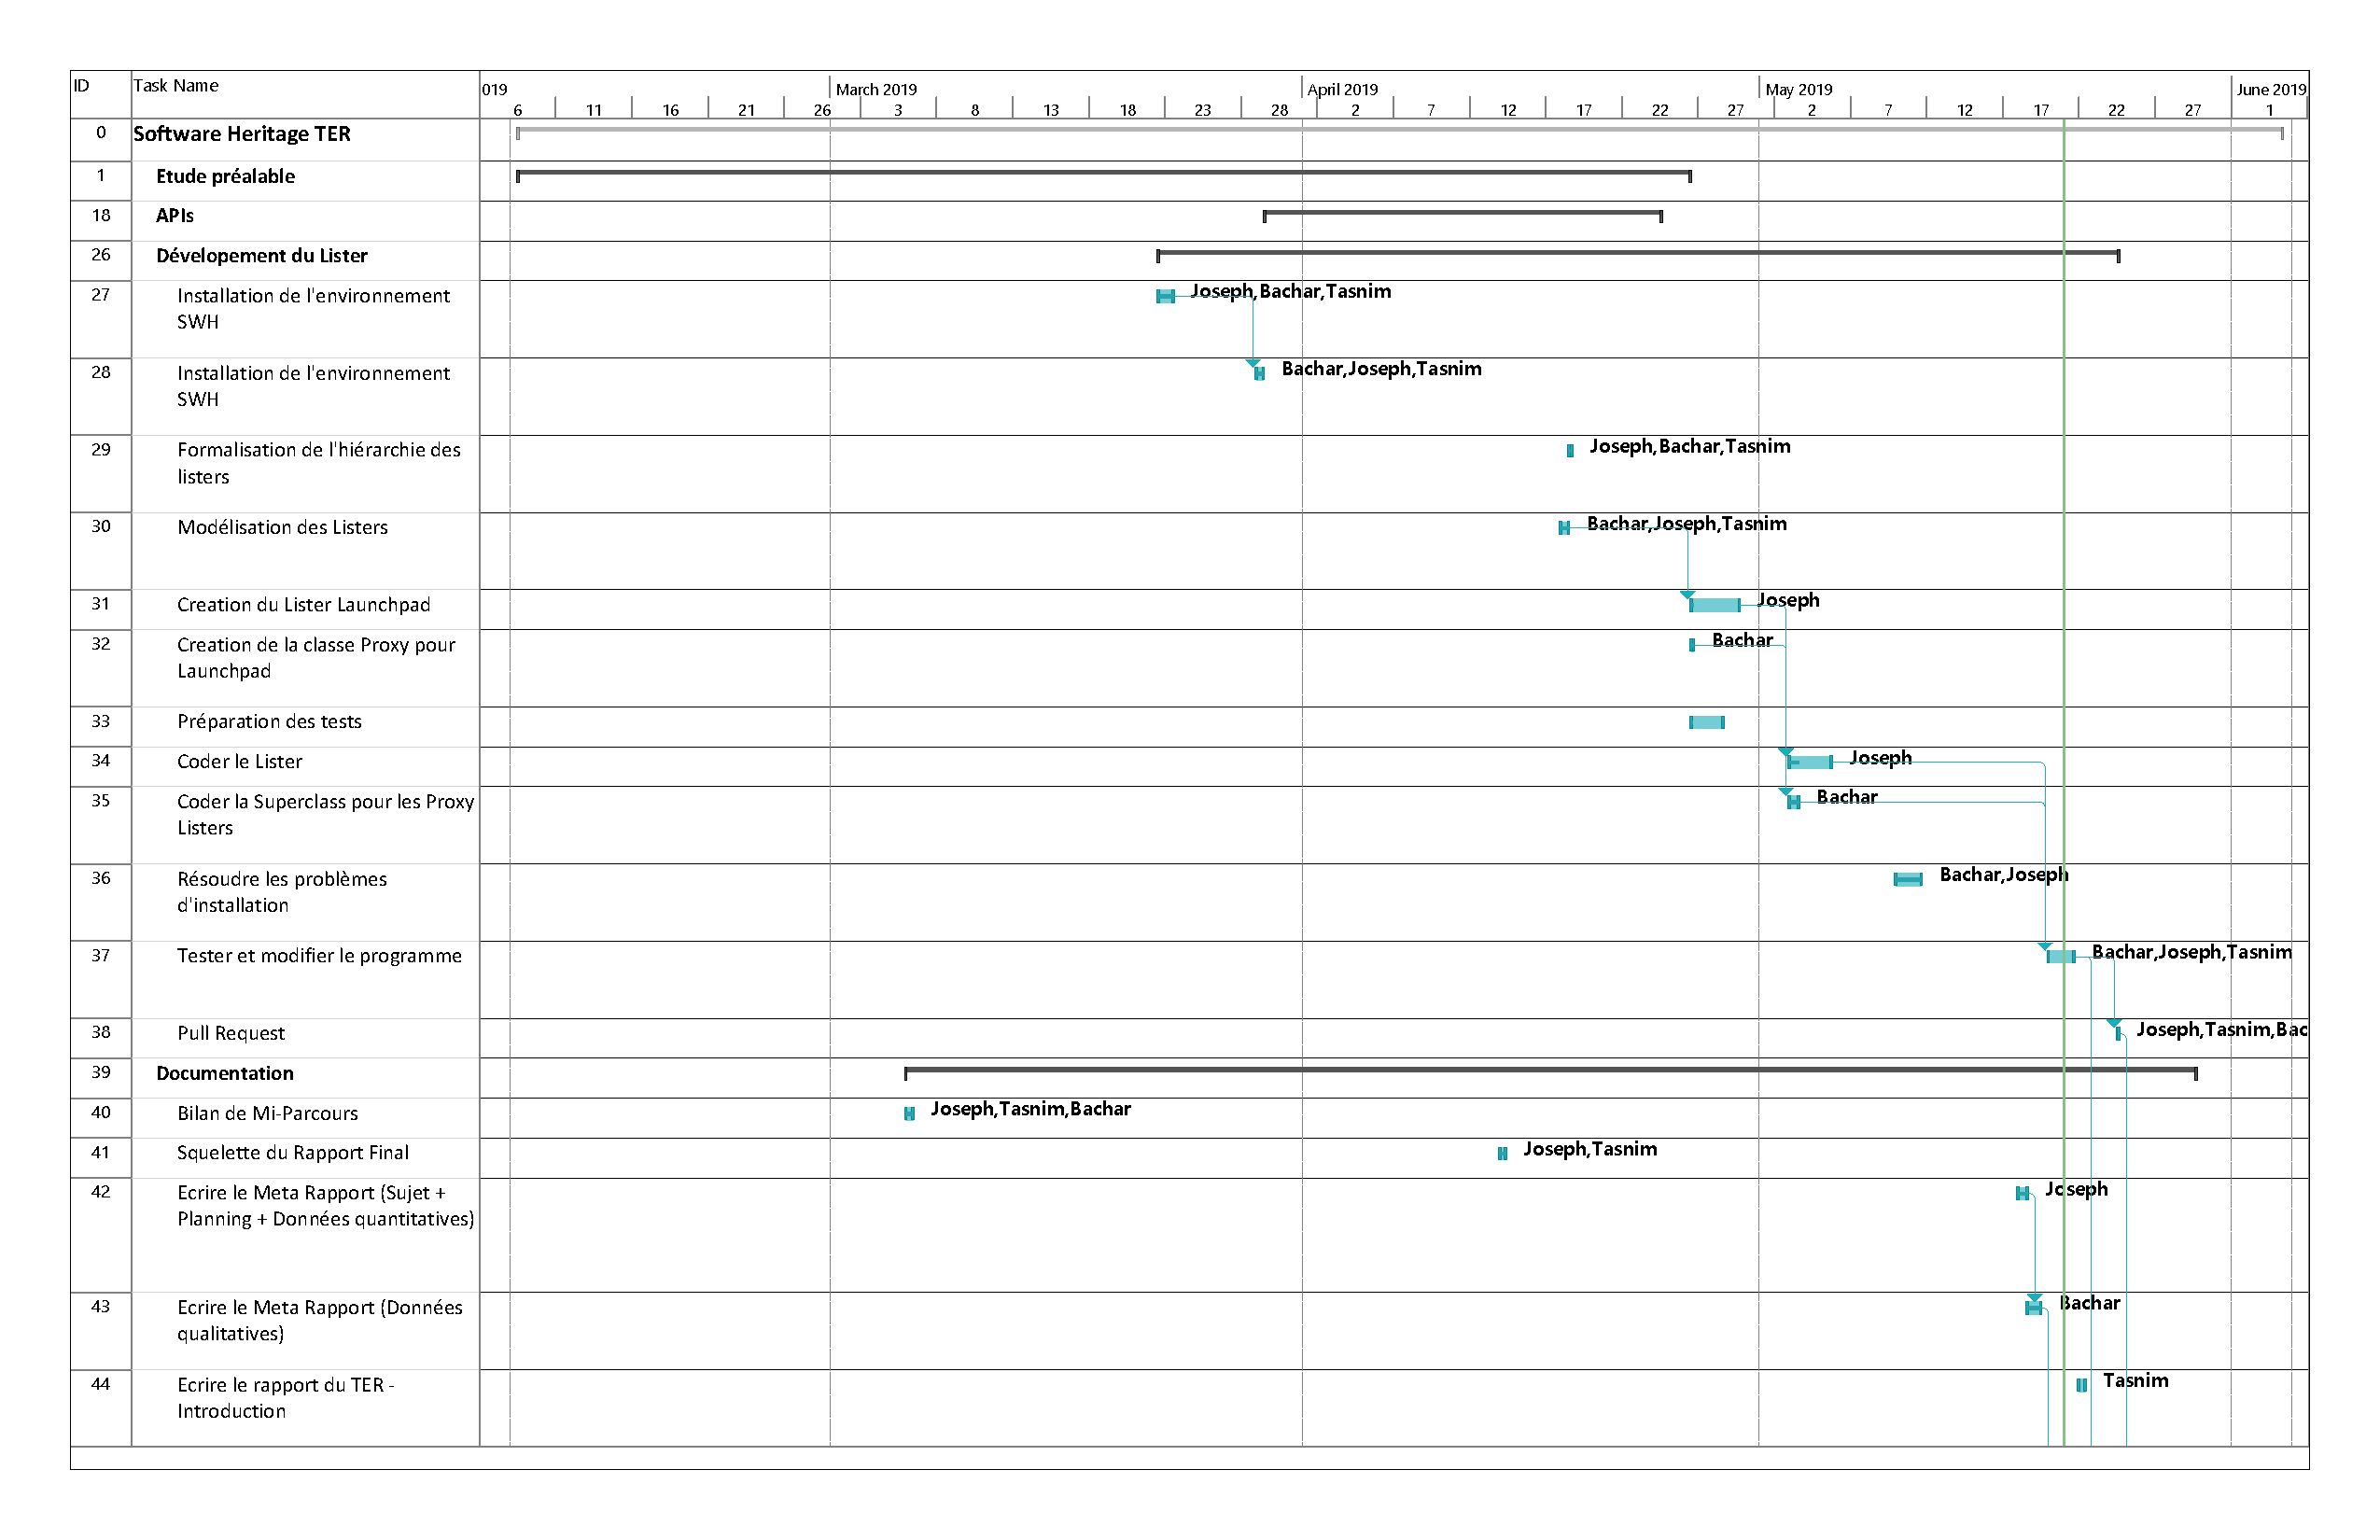
\includegraphics[scale=0.45]{pdfs/planning_final_summary.pdf}
	\end{figure}
	\begin{figure}[!ht]
	\hspace*{-3cm}
	\includegraphics[scale=0.45,page=2]{pdfs/planning_final_summary.pdf}
	\caption{Planning final}
	\end{figure}

	\section{Difficultés rencontrées}
	Au cours de se projet, nous avons rencontrer des difficultés auxquelles nous ne nous attendions pas.
	\subsection{Les APIs}
	\subsection{Les tests}

	\section{Perspectives}
	ce qu'on a fait (extensibilité du code, le fait qu'il est parametrable grace au classes abstraites)
	ce qu'on peut améliorer (les tests? informations du context)
	\section{Bilan et apports du TER}
annexes\\
resumés\\
code

\bibliographystyle{unsrt}
\bibliography{mybib}

\end{document}
